\section{Wiener Kolmogorov Filter}

Verwendung (SNT\_04\_Stoerreduktion, S. 38):
\begin{itemize}
\item reine Rauschbefreiung
\item reine Entzerrung
\item lineare Prädiktion
\end{itemize}

Bei gemeinsam normalverteilten Zufallsvariablen sind lineare Filter optimal.


\textbf{Ursprüngliches Signal:}
\begin{align}
X(n)
\end{align}
\textbf{Signal nach Übertragung:}
\begin{align}
Y(n)
\end{align}
\textbf{Schätzung des Signals:}
\begin{align}
Z(n)
\end{align}
\textbf{Fehler (Differenz):}
\begin{align}
d(n) = X(n) - Z(n)
\end{align}

\textbf{Filtereinstellung:}
\begin{align}
H_{opt}(\Omega) &= \frac{S_{XX}(\Omega)}{S_{XX}(\Omega) + S_{NN}(\Omega)}
\end{align}


\textbf{Orthogonalitätsprinzip:}

Bei einer optimalen Schätzung ist der Fehler orthogonal (senkrecht) zur Schätzung.

\begin{align}
R_{DZ_{opt}}(0) = \mathbb{E}[d(n)Z_{\text{opt}}(n)] &= 0 \\
\Leftrightarrow \mathbb{E}[Z_{\text{opt}}(n)^2] &= \mathbb{E}[X(n) Z_{\text{opt}}(n)]
\end{align}

Besteht das Eingangssignal aus gemeinsam normalverteilten Zufallsvariablen, sind Fehler und Ausgabe dann statistisch unabhängig.

% Final expression for the mean squared error
Beispielrechnung:
\begin{align}
\sigma_d^2 &= \mathbb{E}[(X(n)-Z_{\text{opt}}(n))^2]= \mathbb{E}[X(n)^2 - 2X(n)Z_{\text{opt}}(n) + Z_{\text{opt}}(n)^2] \\
&= \mathbb{E}[X(n)^2-X(n)Z_{\text{opt}}(n)] \quad \text{|Orthogonalitätsprinzip} \\
&= \sigma_X^2 - \sum_{k=1}^{N} h_{k,\text{opt}}R_{XX}(k)\quad \text{| wenn }\mu_X = 0 \\
&= \sigma_X^2 - \mathbf{h}_{\text{opt}}^T\mathbf{r}_{XX}\\
&= \sigma_X^2 - \mathbf{r}_{XX}^T\mathbf{R}_{XX}^{-1}\mathbf{r}_{XX}
\end{align}


\textbf{Rauschbefreiungsfilter:}

\begin{figure}[!htb]
\centering
\begin{tikzpicture}[
    auto, 
    node distance=2cm,
    block/.style={rectangle, draw, minimum height=0.8cm, minimum width=1.2cm},
    mult/.style={rectangle, draw, minimum height=0.8cm, minimum width=0.8cm},
    sum/.style={circle, draw, inner sep=0pt, minimum size=0.7cm},
    >=latex
]
% Neues Eingangssignal X(n) und Noise Addition
\node at (-2,0.3) {$X(n)$};
\node[sum] at (-0.5,0) (noise_sum) {$+$};
\draw[->] (-2,0) -- (noise_sum.west);

% Rauschsignal von unten
\node at (-0.5,-1.3) {$N(n)$};
\draw[->] (-0.5,-1) -- (noise_sum.south);

% Hauptleitung
% Eingangssignal und Verzögerungselemente
\node at (1,0.3) {$Y(n)$};
% Positionierung der Verzögerungselemente
\node[block] at (2.5,0) (delay1) {$z^{-1}$};
\node[block] at (5,0) (delay2) {$z^{-1}$};
\node at (7,0) (dots) {$\cdots$};
\node[block] at (9,0) (delayN) {$z^{-1}$};
% Durchgehende Pfeile, die direkt zu den Boxen führen
\draw[->] (noise_sum.east) -- (delay1.west);
\draw[->] (delay1.east) -- (delay2.west);
\draw[->] (delay2.east) -- (6.4,0);
\draw[->] (7.6,0) -- (delayN.west);
% Multiplizierer mit X Symbol
\node[mult] at (1,-2) (weight0) {$\times$};
\node at (1.8,-2) {$h_0$};
\node[mult] at (3.5,-2) (weight1) {$\times$};
\node at (4.3,-2) {$h_1$};
\node[mult] at (6,-2) (weight2) {$\times$};
\node at (6.8,-2) {$h_2$};
\node[mult] at (10,-2) (weightN) {$\times$};
\node at (10.8,-2) {$h_N$};
% Summierer
\node[sum] at (1,-4) (sum0) {$+$};
\node[sum] at (3.5,-4) (sum1) {$+$};
\node[sum] at (6,-4) (sum2) {$+$};
\node at (7.5,-4) (dots2) {$\cdots$};
\node[sum] at (10,-4) (sumN) {$+$};
% Ausgang
\node at (11.5,-4) (output) {$Z(n)$};
% Vertikale Verbindungen
\draw[->] (1,0) -- (weight0);
\draw[->] (3.5,0) -- (weight1);
\draw[->] (6,0) -- (weight2);
\draw[->] (delayN.east) -- ++(0.4,0) -- ++(0,-1.2) -- (10,-1.2) -- (weightN.north);
% Verbindungen zu Summierern
\draw[->] (weight0) -- (sum0);
\draw[->] (weight1) -- (sum1);
\draw[->] (weight2) -- (sum2);
\draw[->] (weightN) -- (sumN);
% Verbindungen zwischen Summierern
\draw[->] (sum0) -- (sum1);
\draw[->] (sum1) -- (sum2);
\draw[->] (sum2) -- (dots2);
\draw[->] (dots2) -- (sumN);
\draw[->] (sumN) -- (output);
\end{tikzpicture}
\caption{Rauschbefreiungsfilter}
\end{figure}

\FloatBarrier


\begin{align}
Z(n) &= \sum_{k=0}^{N} h_k Y(n-k)
\end{align}
\begin{align}
\min\{MSE\}  \Rightarrow 0 &\overset{!}{=} \frac{\partial MSE}{\partial h_i} = \frac{\partial \mathbb{E}[(X(n)-Z(n))^2]}{\partial h_i}\\
&= \frac{\partial \mathbb{E}[u(v(n))]}{\partial h_i} = \mathbb{E}[u'(v(n)) \cdot v'(n)] = \mathbb{E}[2 \cdot (X(n)-Z(n)) \cdot \frac{\partial v(n)}{\partial h_i}]\\
&= \mathbb{E}[2 \cdot (X(n)-Z(n)) \cdot -Y(n-i)] = -2 \cdot \mathbb{E}[(X(n)-Z(n)) \cdot Y(n-i)]\\
\Rightarrow 0 &= \mathbb{E}[X(n) \cdot Y(n-i)] - \mathbb{E}[Z(n) \cdot Y(n-i)]\\
\Leftrightarrow \mathbb{E}[X(n) \cdot Y(n-i)] &= \mathbb{E}[Z(n) \cdot Y(n-i)]\\
\Leftrightarrow R_{XY}(i) &= \mathbb{E}\left[\sum_{k=0}^{N} h_k Y(n-k) \cdot Y(n-i)\right] = \sum_{k=0}^{N} h_k \cdot \mathbb{E}[Y(n-k) \cdot Y(n-i)]\\
&= \sum_{k=0}^{N} h_k \cdot R_{YY}(i-k)\\
\text{(da, } R_{YY}(-i) = R_{YY}(i) \text{)}\\
\Rightarrow \mathbf{R_{YY}} \cdot \mathbf{h_{\text{opt}}} &= \mathbf{R_{XY}}
\end{align}

% In Matrixform
\begin{align}
\begin{bmatrix}
R_{YY}(0) & R_{YY}(1) \\
R_{YY}(1) & R_{YY}(0)
\end{bmatrix}
\begin{bmatrix}
h_{0,\text{opt}} \\
h_{1,\text{opt}}
\end{bmatrix}
&=
\begin{bmatrix}
R_{XY}(0) \\
R_{XY}(1)
\end{bmatrix}
\end{align}



\text{Filtereinstellung:}
\begin{align}
H_{opt}(\Omega) &=\frac{S_{XY}(\Omega)}{S_{YY}(\Omega)} = \frac{S_{XX}(\Omega)}{S_{XX}(\Omega) + S_{NN}(\Omega)}
\end{align}

\begin{align}
S_{XY}(\Omega) &= \mathcal{F}\{\mathbb{E}[X(n)\cdot Y(n+m)]\} = \mathcal{F}\{\mathbb{E}[X(n)\cdot(X(n+m) + N(n+m))]\}\\
R_{XN}(k) = 0 \Rightarrow \quad S_{XY}(\Omega) &= \mathcal{F}\{\mathbb{E}[X(n)\cdot X(n+m)]\} = S_{XX}(\Omega)
\end{align}
\begin{align}
S_{YY}(\Omega) &= \mathcal{F}\{\mathbb{E}[Y(n)\cdot Y(n+m)]\} = \mathcal{F}\{\mathbb{E}[(X(n) + N(n))\cdot(X(n+m) + N(n+m))]\}\\
R_{XN}(k) = 0 \Rightarrow S_{YY}(\Omega) &= \mathcal{F}\{\mathbb{E}[X(n)\cdot X(n+m)] + \mathbb{E}[N(n)\cdot N(n+m)]\} = S_{XX}(\Omega) + S_{NN}(\Omega)
\end{align}


\textbf{Prädiktionsfilter:}
\begin{figure}[!htb]
\centering
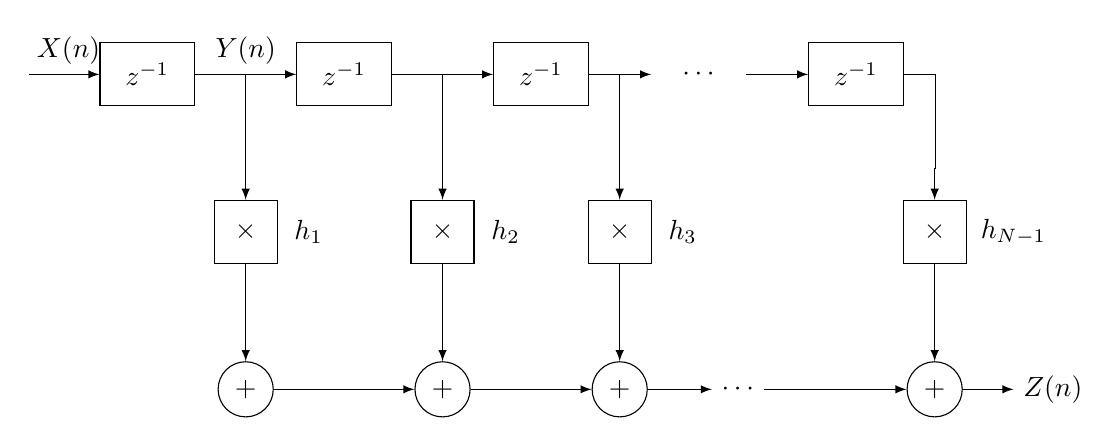
\begin{tikzpicture}[
    auto, 
    node distance=2cm,
    block/.style={rectangle, draw, minimum height=0.8cm, minimum width=1.2cm},
    mult/.style={rectangle, draw, minimum height=0.8cm, minimum width=0.8cm},
    sum/.style={circle, draw, inner sep=0pt, minimum size=0.7cm},
    >=latex
]
% Hauptleitung
% Eingangssignal 
\node at (0.5,0.3) {$X(n)$};

% Erster Verzögerungsblock für Prädiktion
\node[block] at (1.5,0) (pred) {$z^{-1}$};
\draw[->] (0,0) -- (pred.west);

% y(n) nach dem ersten z^{-1} Element
\node at (2.75,0.3) {$Y(n)$};

% Verzögerungselemente nach der Prädiktion
\node[block] at (4,0) (delay1) {$z^{-1}$};
\node[block] at (6.5,0) (delay2) {$z^{-1}$};
\node at (8.5,0) (dots) {$\cdots$};
\node[block] at (10.5,0) (delayN) {$z^{-1}$};

% Durchgehende Pfeile, die direkt zu den Boxen führen
\draw[->] (pred.east) -- (delay1.west);
\draw[->] (delay1.east) -- (delay2.west);
\draw[->] (delay2.east) -- (7.9,0);
\draw[->] (9.1,0) -- (delayN.west);

% Multiplizierer mit X Symbol
\node[mult] at (2.75,-2) (weight0) {$\times$};
\node at (3.55,-2) {$h_1$};
\node[mult] at (5.25,-2) (weight1) {$\times$};
\node at (6.05,-2) {$h_2$};
\node[mult] at (7.5,-2) (weight2) {$\times$};
\node at (8.3,-2) {$h_3$};
\node[mult] at (11.5,-2) (weightN) {$\times$};
\node at (12.5,-2) {$h_{N-1}$};

% Summierer
\node[sum] at (2.75,-4) (sum0) {$+$};
\node[sum] at (5.25,-4) (sum1) {$+$};
\node[sum] at (7.5,-4) (sum2) {$+$};
\node at (9,-4) (dots2) {$\cdots$};
\node[sum] at (11.5,-4) (sumN) {$+$};

% Ausgang
\node at (13,-4) (output) {$Z(n)$};

% Vertikale Verbindungen
\draw[->] (2.75,0) -- (weight0);
\draw[->] (5.25,0) -- (weight1);
\draw[->] (7.5,0) -- (weight2);
\draw[->] (delayN.east) -- ++(0.4,0) -- ++(0,-1.2) -- (11.5,-1.2) -- (weightN.north);

% Verbindungen zu Summierern
\draw[->] (weight0) -- (sum0);
\draw[->] (weight1) -- (sum1);
\draw[->] (weight2) -- (sum2);
\draw[->] (weightN) -- (sumN);

% Verbindungen zwischen Summierern
\draw[->] (sum0) -- (sum1);
\draw[->] (sum1) -- (sum2);
\draw[->] (sum2) -- (dots2);
\draw[->] (dots2) -- (sumN);
\draw[->] (sumN) -- (output);
\end{tikzpicture}
\caption{Prädiktionsfilter}
\end{figure}

\FloatBarrier

\begin{align}
Z(n) &= \sum_{k=1}^{N} h_k X(n-k)
\end{align}

% Matrix für Prädiktionsfilter
\begin{align}
\begin{bmatrix}
R_{XX}(0) & R_{XX}(1) \\
R_{XX}(1) & R_{XX}(0)
\end{bmatrix}
\begin{bmatrix}
h_{1,\text{opt}} \\
h_{2,\text{opt}}
\end{bmatrix}
=
\begin{bmatrix}
R_{XX}(1) \\
R_{XX}(2)
\end{bmatrix}
\end{align}

\begin{align}
\mathbf{R_{XX}} \cdot \mathbf{h_{\text{opt}}} &=
\begin{bmatrix}
R_{XX}(1) \\
R_{XX}(2)
\end{bmatrix}
\end{align}

\begin{align}
\min\{\sigma_d^2\} &= \sigma_x^2 - \sum_{k} h_k R_{XX}(k)
\end{align}



\textbf{LTI System:}
\begin{figure}[ht]
\centering
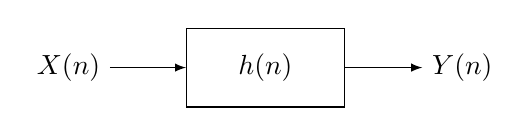
\begin{tikzpicture}[
    auto, 
    node distance=2cm,
    block/.style={rectangle, draw, minimum height=1cm, minimum width=2cm},
    >=latex
]
% Elemente des linearen Systems
\node at (0,0) (input) {$X(n)$};
\node[block] at (2.5,0) (system) {$h(n)$};
\node at (5,0) (output) {$Y(n)$};

% Verbindungspfeile
\draw[->] (input) -- (system);
\draw[->] (system) -- (output);
\end{tikzpicture}
\end{figure}

\FloatBarrier

Frequenzbereich - Multiplikation:
\begin{align}
Y(n) = X(n) * h(n) = h(n) * X(n); Y(j\Omega) = X(j\Omega) \cdot H(j\Omega)
\end{align}

Leistungsdichtespektrum:
\begin{align}
S_{YY}(\Omega) = S_{XX}(\Omega) \cdot |H(j\Omega)|^2
\end{align}

Zusammenhang durch Fourier-Transformation:
Darstellung des Fourier-Transformation:
\begin{align}
h(n) \overset{\mathcal{F}}{\circ\mbox{---}\bullet} H(j\Omega)
\end{align}
\begin{align}
H(j\Omega) &= \mathcal{F}\{h(n)\} = \sum_{n=-\infty}^{\infty} h(n) e^{-j\Omega n} \\
h(n) &= \mathcal{F}^{-1}\{H(j\Omega)\} = \frac{1}{2\pi} \int_{-\pi}^{\pi} H(j\Omega) e^{j\Omega n} \, d\Omega
\end{align}


\textbf{Faltungsrechenregeln:}
\begin{align}
X(n) * \delta(n) = X(n)
\end{align}
\begin{align}
X(n) * \delta(n-m) = X(n-m)
\end{align}
\begin{align}
X(n) * [a \cdot h(n)] = a \cdot [X(n) * h(n)]
\end{align}
\begin{align}
X(j\Omega) \cdot [a \cdot H(j\Omega)] = a \cdot [X(j\Omega) \cdot H(j\Omega)]
\end{align}
